\chapter{議論}
前章までにおいて,\$Vアルゴリズム及び性能評価を述べた.
本章において,\$Vが今後どのように改善されうるか,あるいは\$Vをどのように発展利用できるかについて議論する.

\section{最適な重み付けの再定義}
5.4節において,認識率及びN-best Lists の1番目と2番目のスコアの差を向上させるための最適な重みを実験的に求めた.
しかしながら,ジェスチャグループ内の学習データ間の類似度と最適な重みの関係を示す近似式の決定係数$R^2$は高いとは言えず,今回は,式〜において示されるように定数を1つにし,段階的に変化させることによって近似式を求めた.
このように決定係数$R^2$が低くなった要因は,ジェスチャグループ内の学習データ間の類似度と最適な重みにおいてある程度相関を示したものの,元データにばらつきが多く存在することであると考えられる.

今回,この元データは,あるジェスチャグループ内の学習データ間の類似度において,ジェスチャが一致した時の類似度の平均値が0.9以上,N-best Listの1番目と2番目のスコアの差が0.2以上の時のそれぞれの特徴量に対する重みの平均値としてプロットされている.しかしながら,当然ながらこの条件を満たす多くの重みにおいて,具体的な類似度の平均値及びN-best Listの1番目と2番目のスコアの差には違いがある~(例えば,類似度が0.9,N-best Listの1番目と2番目のスコアの差が0.2である重みも存在すれば,類似度が0.99,N-best Listの1番目と2番目のスコアの差が0.4である重みも存在する).このことから,条件を満たす重みを平均するのではなく,高いスコアを示す重みをより重要視することによって,データのばらつきを抑えられる可能性がある.
データのばらつきを抑えることによって,近似式の決定係数$R^2$は高くなり,より元データを忠実に表す近似式を得られ,認識率の向上あるいは識別能力の向上を実現できるかもしれない.


\section{ユーザに依存しない手書きジェスチャの精度評価}
本論文において,ジェスチャを定義したアプリケーションユーザが,自身が定義したジェスチャを入力した時に,\$Vがどれだけ認識できるか,あるいはどれだけ識別できるかを評価した.今回はアプリケーションユーザが定義する場合を想定しているため,このように,ユーザに依存した手書きジェスチャの評価を行った.しかしながら,アプリケーション開発者が手書きジェスチャを定義する場合,実際に入力するのはアプリケーションユーザであるため,ユーザに依存しない手書きジェスチャにおいても,高い認識率及び高い識別性能が求められる.\$Vはロバスト性を極力維持するために,識別に必要のない特徴量の重みを小さくするなどの処理を施しているため,ユーザに依存しない手書きジェスチャにおいて,
重み付けをしない場合と比べて,高い認識率及び高い識別能力を示す可能性が高い.\$1,DTW,Rubineとの比較を含め,ユーザに依存しない手書きジェスチャの精度評価を行うことによって,さらなる改善の余地を発見するかもしれない.


\section{書き順に依存しないアルゴリズムの導入}
\$Vは\$1の拡張であり,\$1と同様に形状と書き順を同じジェスチャを認識することができるため,図\ref{fig:different_direction}のような形状が同じであっても書き順の異なるジェスチャは別のジェスチャとして認識される.双方を同じジェスチャとして認識してほしい場合には,それぞれのジェスチャを同じ名前で登録する必要がある.
このようなアプリケーションユーザへの負担を解消すべく,書き順に依存しない,つまり形状さえ同じであれば同じジェスチャとみなすアルゴリズムは\$N~\cite{}において開発されているため,このアルゴリズムを活用することによって書き順に依存しないアルゴリズムを実現することができる.

\begin{figure} [h!]
	\begin{center}
		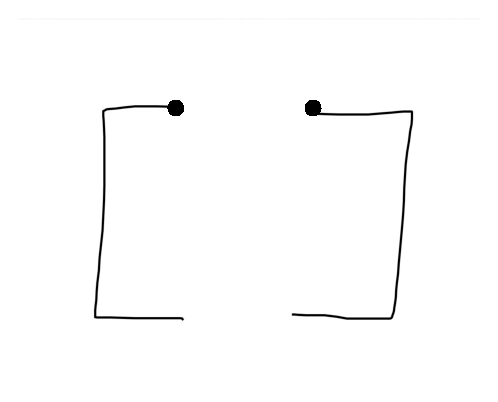
\includegraphics [width=0.5\hsize ]{img/different_direction.eps}
	\end{center}
	\caption{形状が同じであるが書き順の異なる手書きジェスチャの例}
	\label{fig:different_direction}
\end{figure}


\section{スマートフォン以外の端末への応用}
\$Vは,スマートフォンへの手書きジェスチャの入力を想定した,手書きジェスチャ認識アルゴリズムである.
そのため,スマートフォン以外の端末,例えばスマートウォッチやテーブルトップ端末などへの手書きジェスチャの認識アルゴリズムとしても応用できる.
しかしながら,\$1とは違い,大きさ,向き,位置に関して識別可能であるため,それぞれに対する最適な重みを定義する必要がある.
例えば,スマートウォッチはスマートフォンと比べ入力領域が小さいため,大きさや位置の違いを利用しづらく,大きさや位置への重みが小さくなる可能性が高い,反対に,テーブルトップ端末はスマートフォンと比べ入力領域が大きいため,大きさや位置の違いを利用しやすく,大きさや位置への重みが大きくなる可能性が高い.

このように,入力領域を変数として,最適な重みを定義することによって,スマートフォン以外の端末への大きさ,向き,位置の違いを利用した手書きジェスチャを認識することが可能になる.

\section{空中手書きジェスチャへの応用}
\$Vは,スマートフォンのような端末への入力を想定しており,認識できる手書きジェスチャは2次元のストロークからなる手書きジェスチャである.これを3次元に応用することによって,空中手書きジェスチャを認識することが可能になる.\$3~\cite{}は\$1を3次元に応用し,空中手書きジェスチャを認識可能にした.このアルゴリズムを活用することによって実現することができる.


